\documentclass[a4paper,11pt]{article}


\title{MA3H0 Assignment 2}
\author{Joshua Rydell}
\usepackage{graphicx}
\usepackage{framed}
\usepackage{amsmath}
\usepackage{amssymb}
\usepackage{amsfonts}
\usepackage{cite}
\usepackage{mathrsfs}
\usepackage{array}
\usepackage[numbers]{natbib}
\usepackage[colorlinks=true, urlcolor=blue, linkcolor=red]{hyperref}
\bibliographystyle{plainnat}
\usepackage{cite}

\usepackage{amsthm} %  package used to make the theorem environments work.
% code below sets up new theorem environments
\theoremstyle{plain} % this sets the style for all new environments created using \newtheorem to have the "theorem" style, which as a bold title, italic text and vertical space above and below it. 
\newtheorem{thm}{Theorem}[section] 
\newtheorem{lem}[thm]{Lemma} 
\newtheorem{prop}[thm]{Proposition} 
\newtheorem*{cor}{Corollary} 
\newtheorem*{claim}{Claim} 

\theoremstyle{definition} % this sets the style for all new environments created using \newtheorem to have the "definition" style, which as a bold title, upright text and vertical space above and below it.
\newtheorem{defn}{Definition}[section]
\newtheorem{eg}{Example}[section]


\theoremstyle{remark} % this sets the style for all new environments created using \newtheorem to have the "remark" style, which as an italic non-bold title, upright text and no extra vertical space above and below it.
\newtheorem*{rem}{Remark} 
\newtheorem{case}{Case}

% note that there is already an in-built "proof" environment which we do not need to create


\newcommand{\N}{\mathbb{N}}
\newcommand{\Lc}{\mathcal{L}}
\newcommand{\brac}[1]{\left ( #1  \right )}
\newcommand{\abs}[1]{\left | #1  \right | }
\begin{document}  
\maketitle
\begin{enumerate}
\item We make a mesh a mesh using points from the pygmsh library. We then apply the 
\href{'https://en.wikipedia.org/wiki/Bowyer\%E2\%80\%93Watson_algorithm#:~:text=In\%20computational\%20geometry\%2C\%20the\%20Bowyer,graph\%20of\%20the\%20Delaunay\%20triangulation.}{Bowyer-Watson algorithm} to make a triangulation from these points. The red dot is my choice of, $x_K$, which is the centroid of the each triangle :  

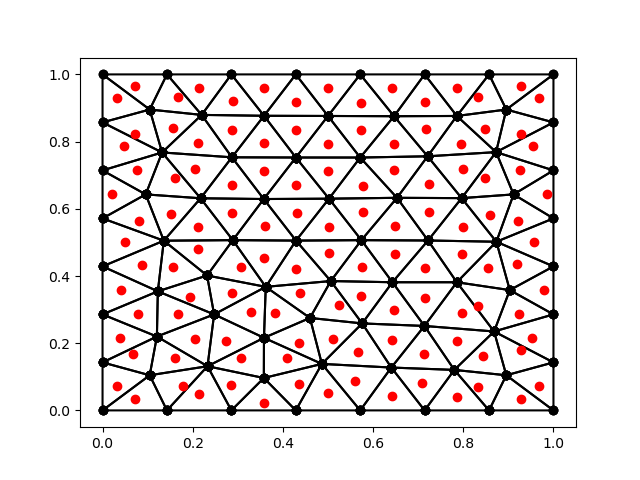
\includegraphics[scale = 0.9]{mesh.png}

\item My choice of $f$ was $f(x,y) = y(1-y)x^3$. I decided to implement my estimate via
\[\frac{1}{m(K)} \int_K f(x) dx \approx f(x_k) \]
this is implemented when we solve the for the system to find the matrix $A$ :
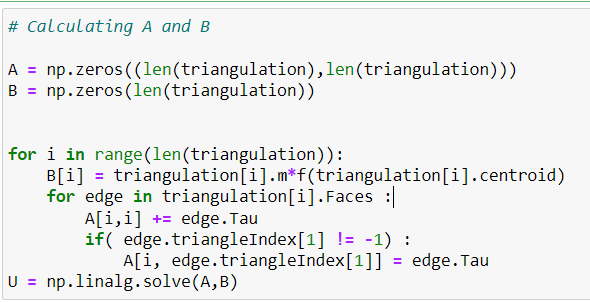
\includegraphics[scale=0.9]{fk.png}
\item I implement the Tau in the Face class:


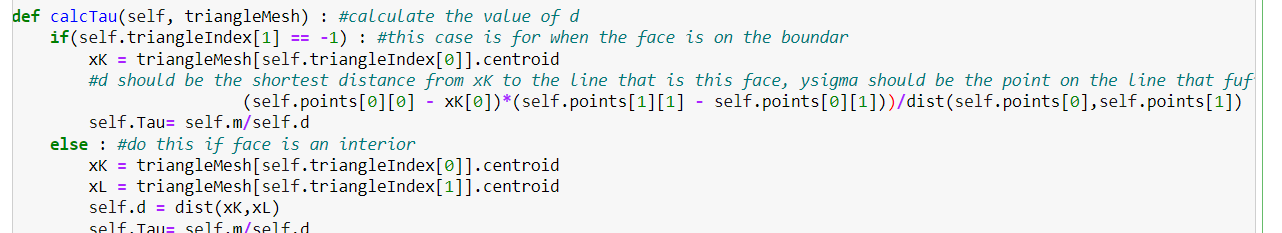
\includegraphics[scale=0.5]{Tau}
\item

\item Let us enumerate the triangles. We write $A = a_{ij}$ and $B = b_i$. We have $b_i = m(T_i)f_{T_i}$, where $i = 0, \dotsc, \#\mathcal{T}$.  Moving on to calculating $A$, we see that each Row of $A$ will have three or four entries. Consider a triangle $T_i$. Suppose $T_i$ is an internal triangle and that $T_i$ shares a face with triangles
$T_{k_1},T_{k_2},T_{k_3}$ then $a_{ik_\ell} =  \tau_{T_i | T_{{k_\ell}}}$ where $\ell = 1,2,3$ and $a_{ii} = \sum_{\ell = 1}^3-\tau_{T_i | T_{k_\ell}}$.

If $T_i$ is on the border then suppose it still shares a border with $T_{k_1},T_{k_2}$, then we still have $a_{ik_\ell} =  \tau_{T_i | T_{k_\ell}}$ where $\ell = 1,2$, but $a_{ii} = \sum_{\ell = 1}^2\tau_{T_i | T_{k_\ell}} + \tau_{i, \sigma}$. Where $\sigma$ is the border edge.

These matrices give us the linearised form of problem (2), so we can write $AU = B$.


\end{enumerate}

\end{document}

